\documentclass[../main.tex]{subfiles}
\begin{document}

\section{Setup}

In this paper we explore whether embeddings of Co-Trajectories as high-dimensional time-location vectors can be used to differentiate large scale movement patterns from mobile network data. Two cases are considered. The first spans the full month of February 2023, and the second Thursdays across 2022. We limit ourselves to a geographic area around Stockholm defined by the bounding box [(59.1000, 18.3400), (59.5000, 17.7300)]. During the dates under study this area contains roughly 3000 antennas, the distribution of which can be seen in figure \ref{fig:antenna_dist}.

The original data was sampled at five minute intervals but to keep pre-processing times reasonable we choose to aggregate samples into hours.
This trade-off seemed reasonable since the focus in question was on large scale movement patterns which would likely remain visible at this lower resolution. Doing this, we also keep the dimension of the vectors lower, since otherwise keeping to 5 minute intervals would result in vectors of size $288 * 3000 = 864000$. 

For each case a pairwise comparison of the vectors were made using both L1, weighted Jaccard metrics. The results are presented as distance matrices and as dendrograms. See figures \ref{fig:feb-dist-dend}, \ref{fig:thu-L1} and \ref{fig:thu-Jaccard}.

As a further visualization we created "movement profiles" for each date and presented them together as heatmaps. See figure \ref{fig:mov-pro-feb} and \ref{fig:full-mov-pro}. Here, instead of comparing dates we instead apply the metrics to compare consecutive hours within a date, creating a rough measure of how 
the device distributions changed throughout the day.
 
Finally we showcase a set of MinHash approximations for larger and larger sample sizes, showing how it approaches the weighted Jaccard metric.

\section{Distance Matrices, Dendrograms, Movement Profiles and MinHashes.}

\begin{figure*}[ht]
\centering
\begin{adjustbox}{center}
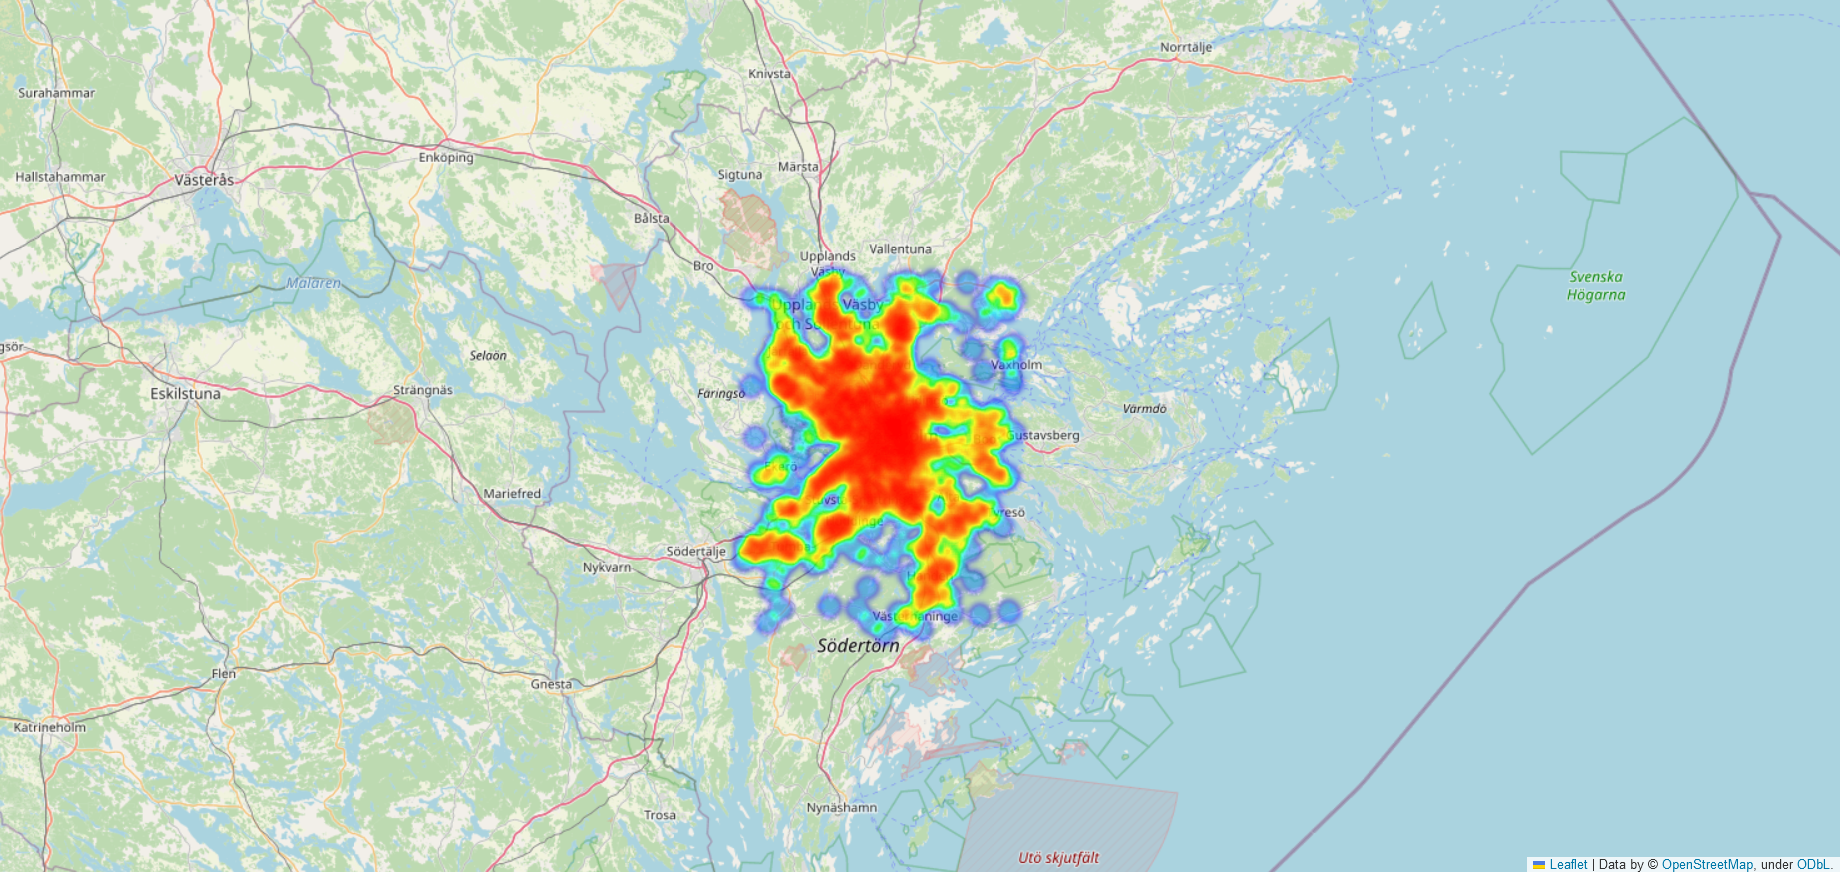
\includegraphics[width=1.2\textwidth]{graphics/results/antenna_distribution.png}
\end{adjustbox}
\caption{Distribution of antennas around Stockholm.}
\label{fig:antenna_dist}
\end{figure*}

\begin{figure*}[ht]
\centering
\begin{adjustbox}{center}
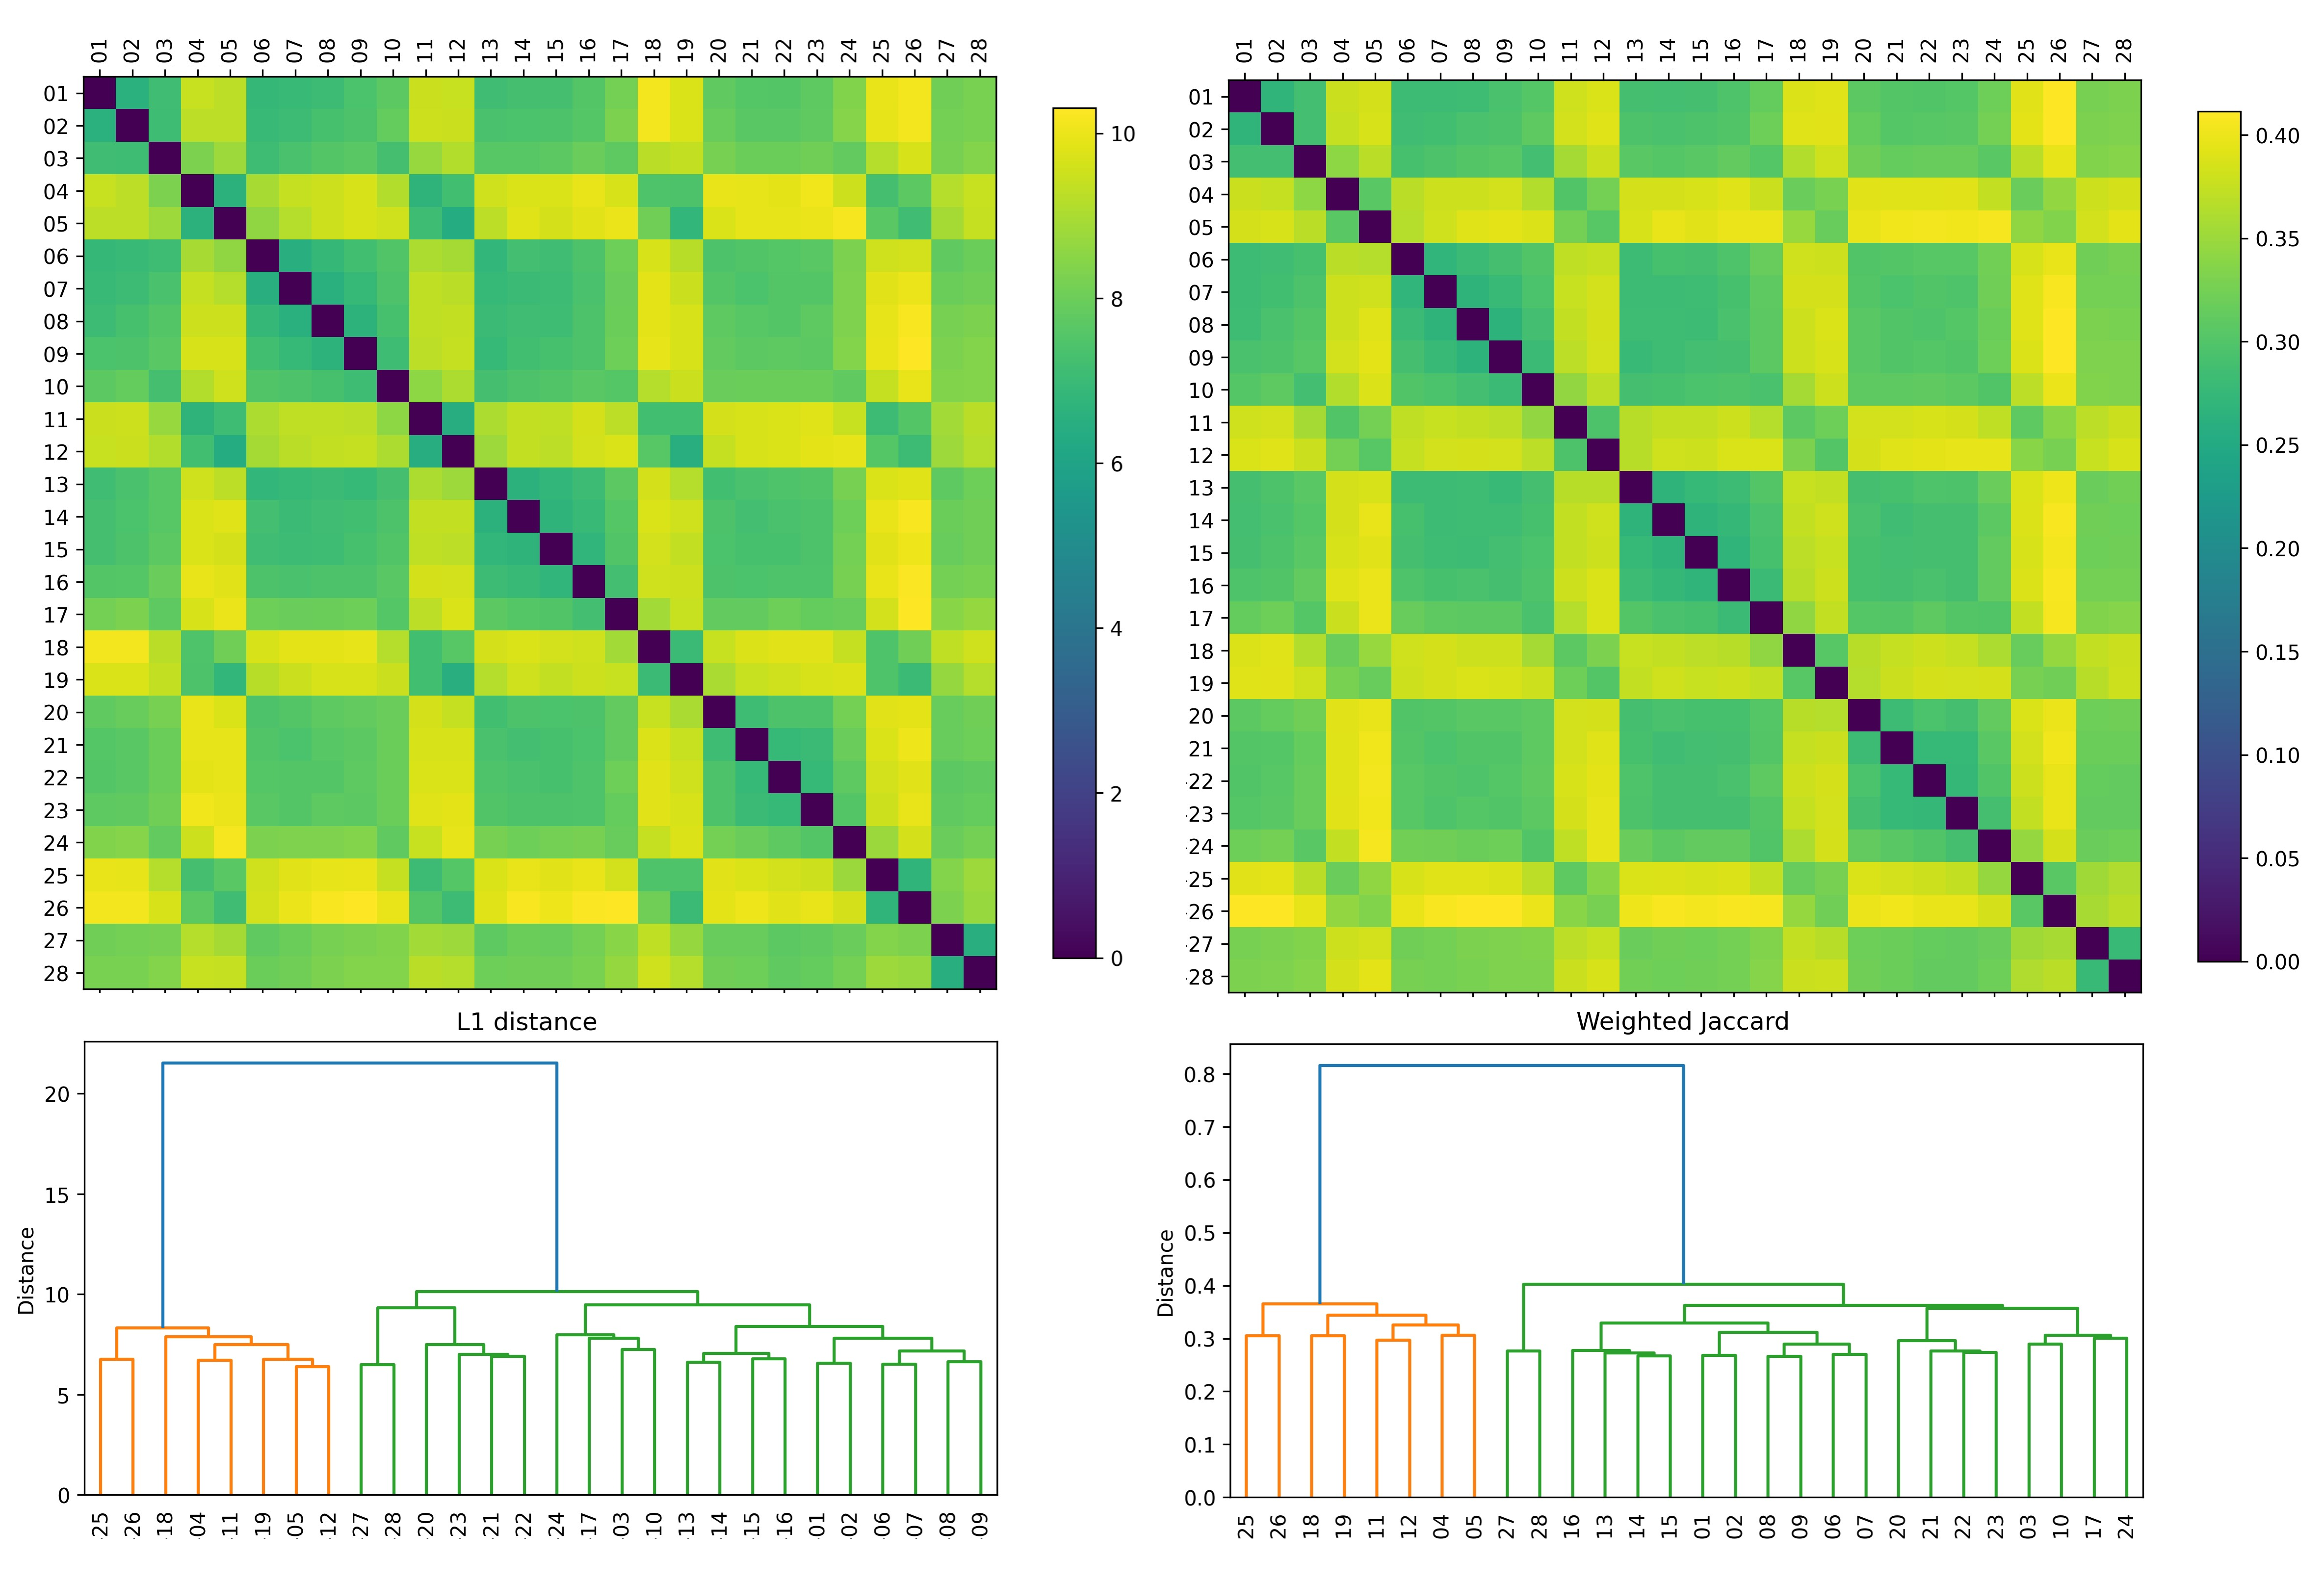
\includegraphics[width=1.6\textwidth]{graphics/results/L1_Jaccard_Feb.png}
\end{adjustbox}
\caption{Distance matrices and dendrograms comparing dates in February 2023 using L1 and Weighted Jaccard distance measures.}
\label{fig:feb-dist-dend}
\end{figure*}

\begin{figure*}[ht]
\centering
\vspace{-30mm}
\begin{adjustbox}{center}
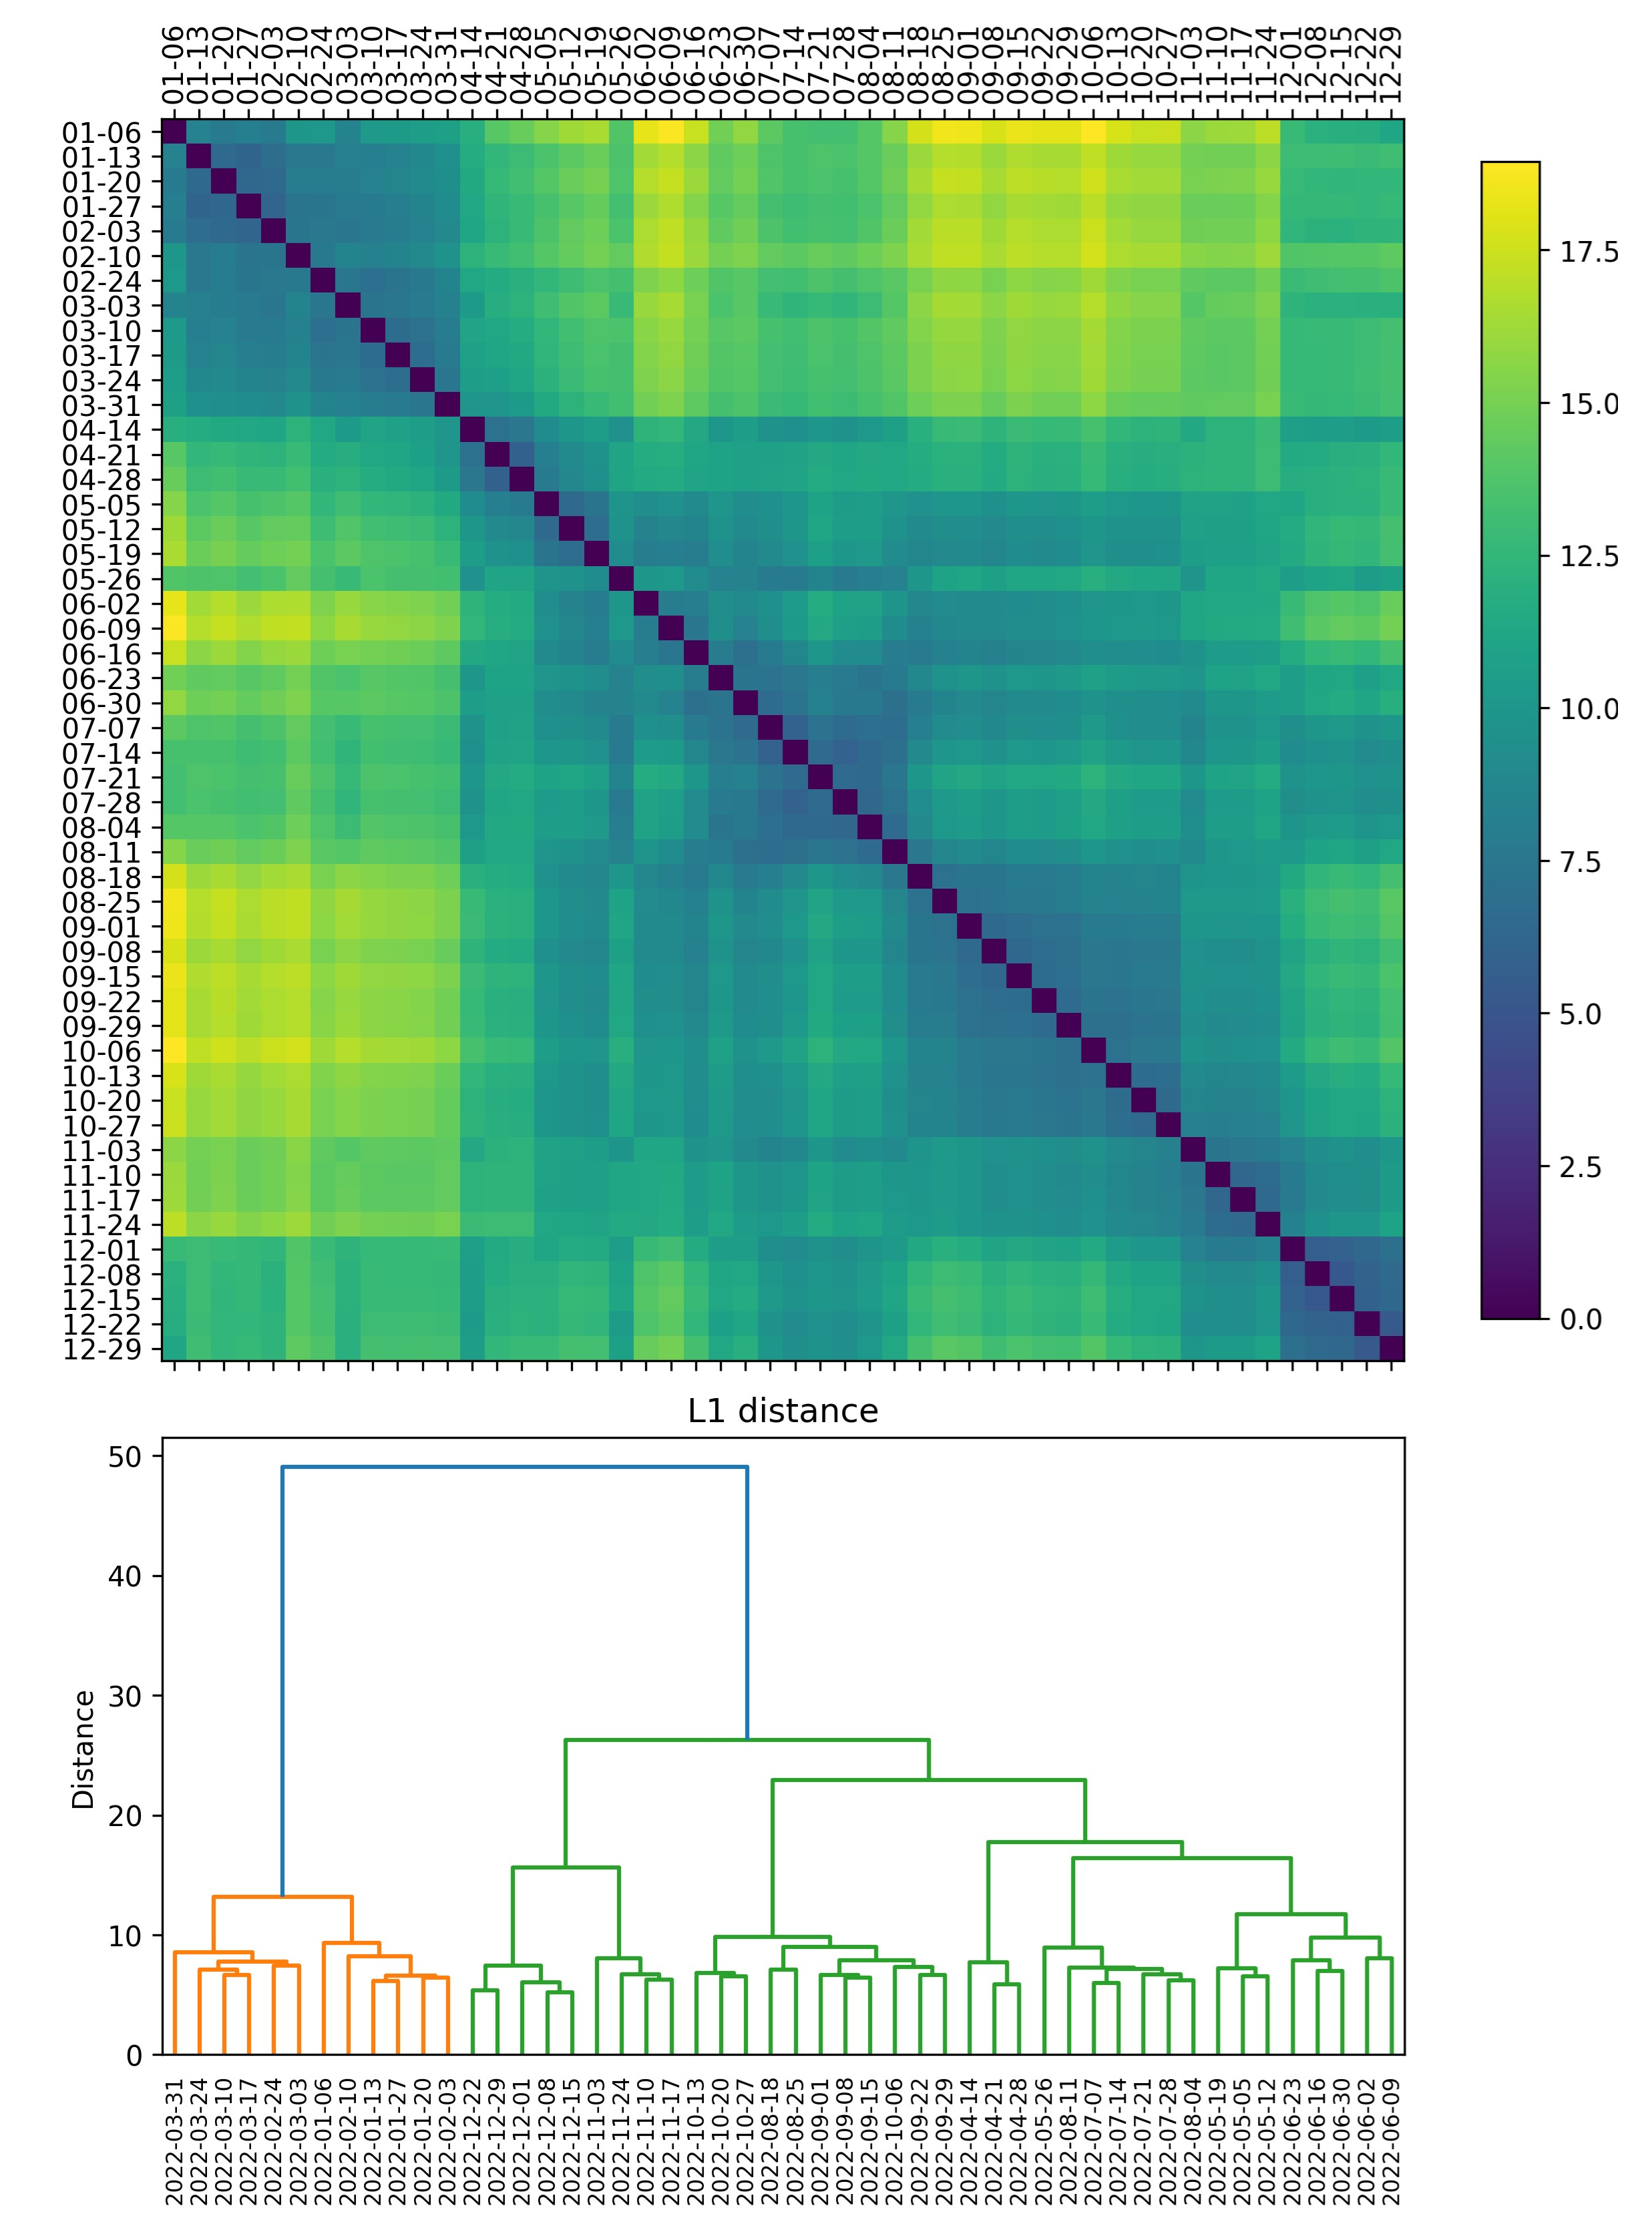
\includegraphics[width=1.3\textwidth]{graphics/results/L1_Thu.png}
\end{adjustbox}
\caption{Distance matrix and dendrogram comparing Thursdays across 2022 using the L1 distance.}
\label{fig:thu-L1}
\end{figure*}

\begin{figure*}[ht]

\centering
\vspace{-30mm}
\begin{adjustbox}{center}
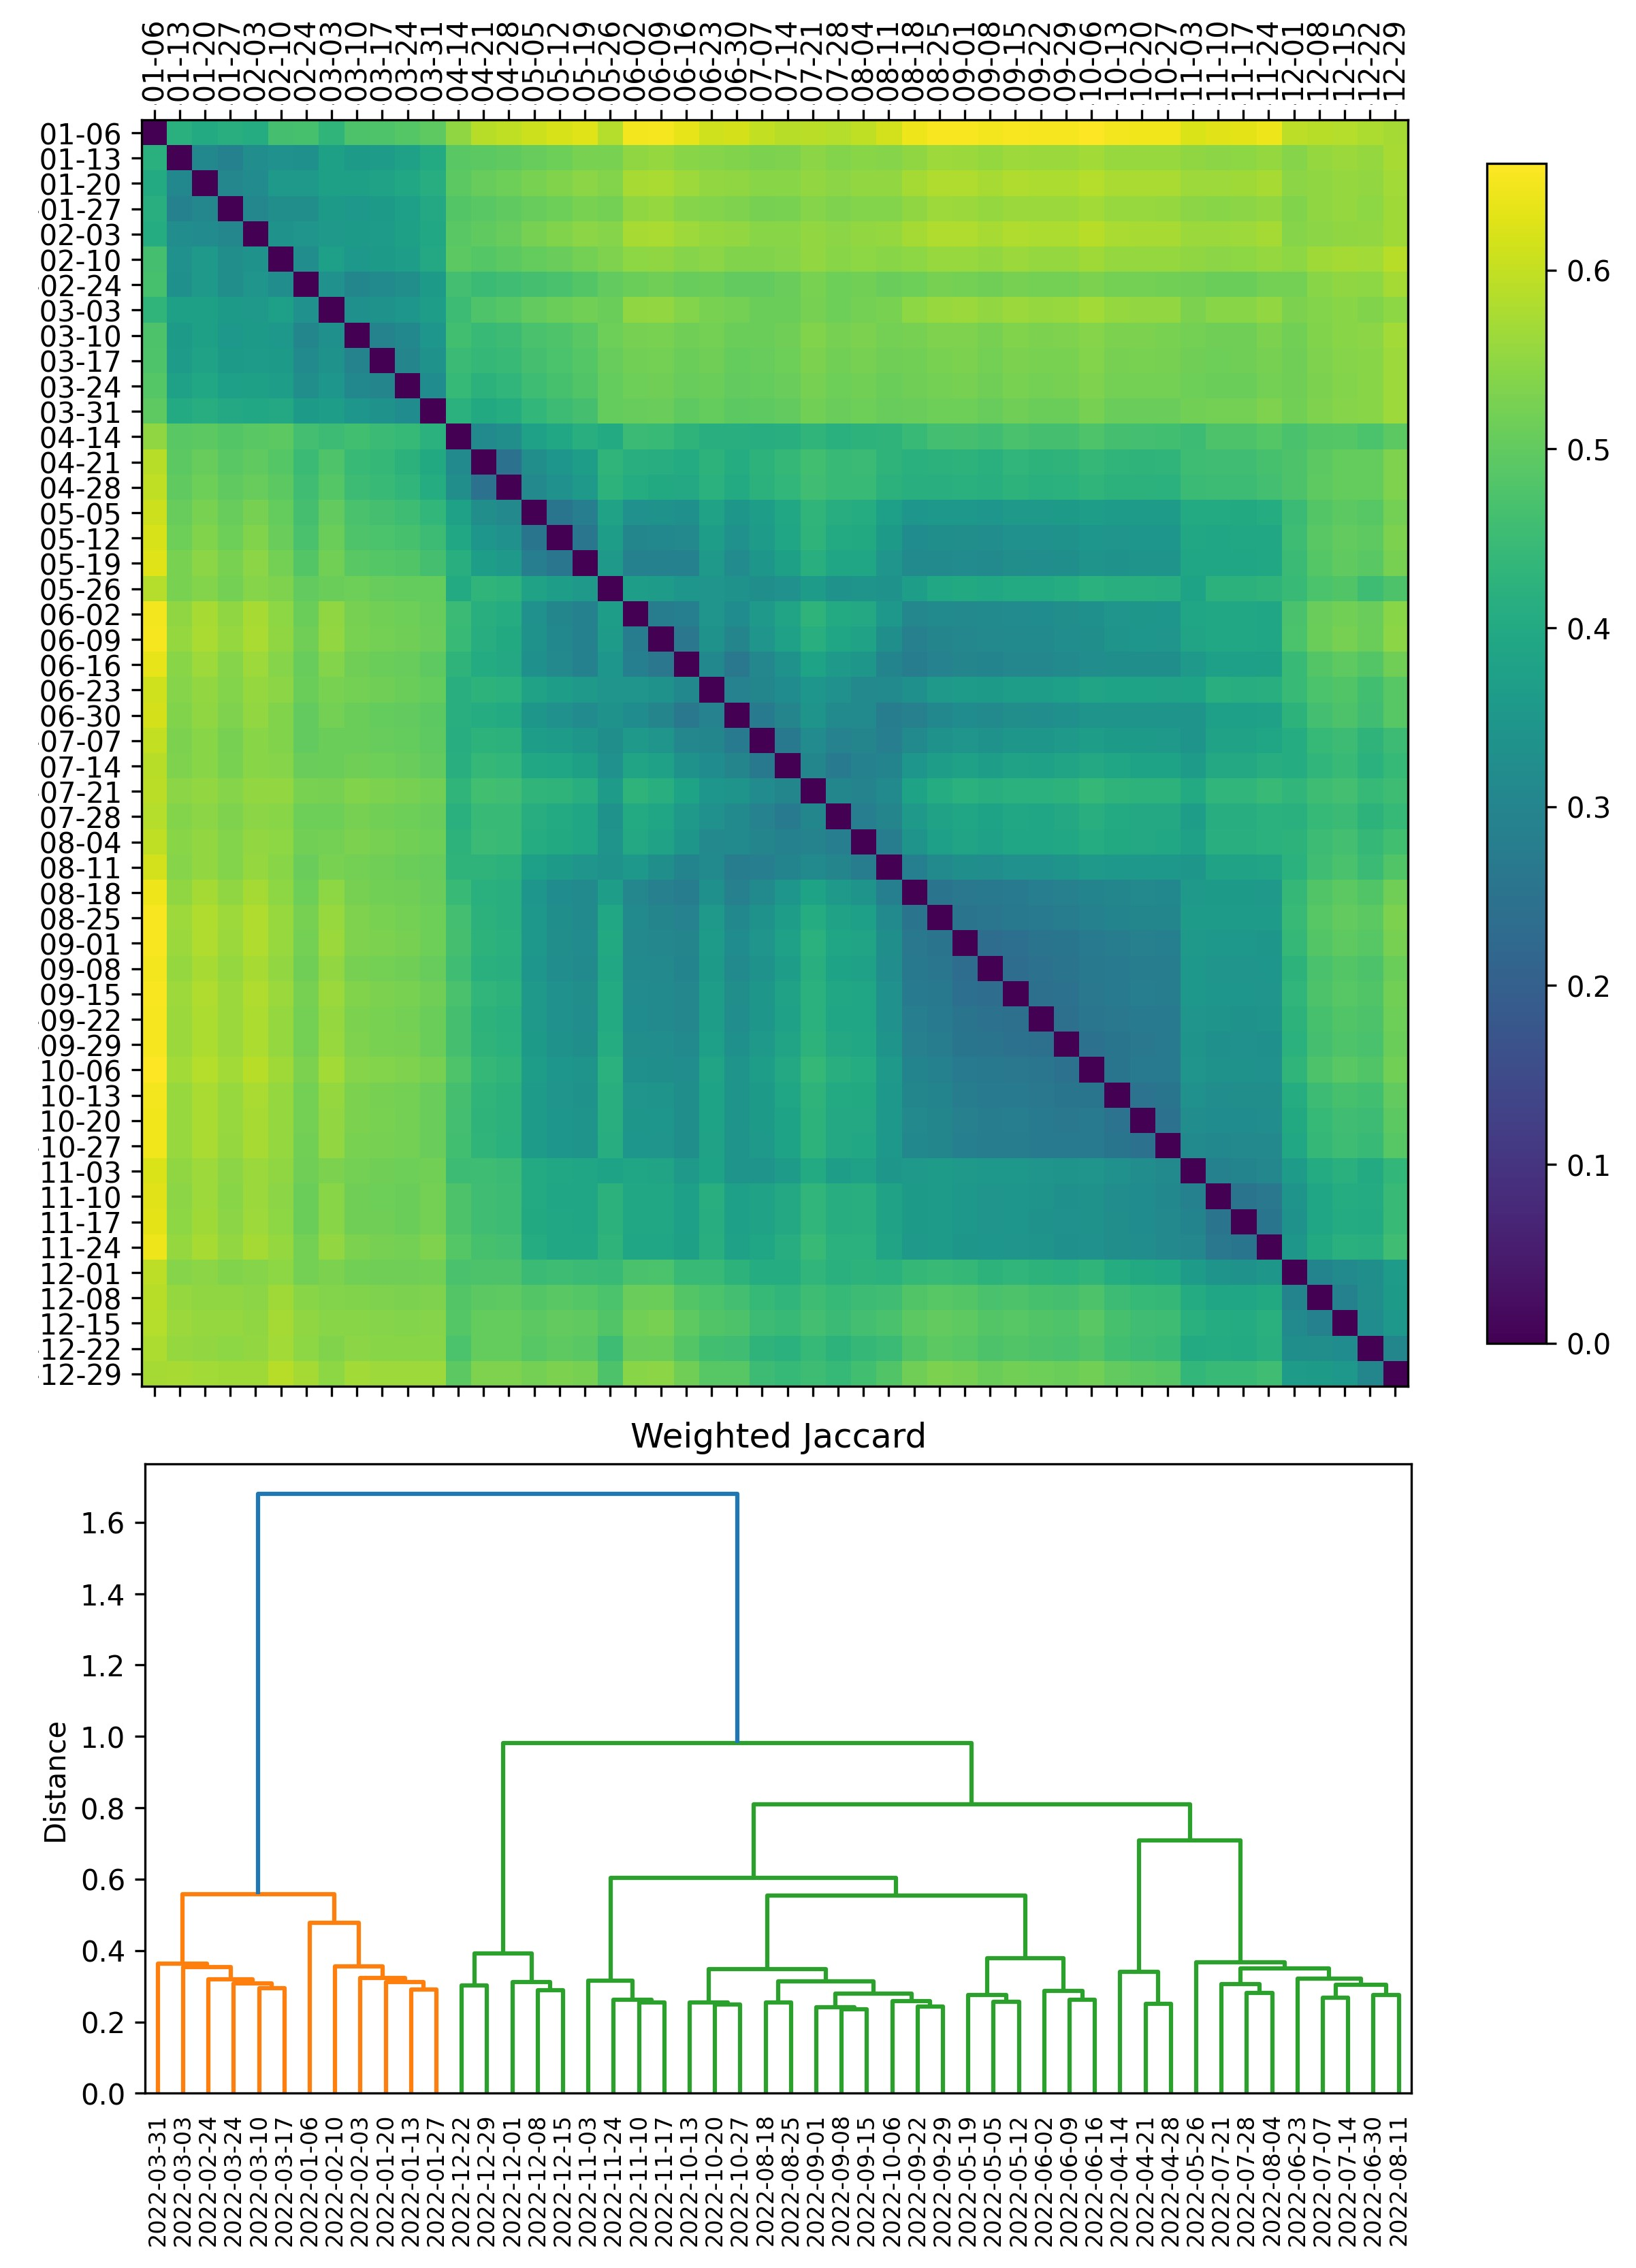
\includegraphics[width=1.3\textwidth]{graphics/results/Jaccard_Thu.png}
\end{adjustbox}
\caption{Distance matrix and dendrogram comparing Thursdays across 2022 using the weighted Jaccard distance.}
\label{fig:thu-Jaccard}
\end{figure*}

\begin{figure*}[ht]
\centering
\begin{adjustbox}{center}
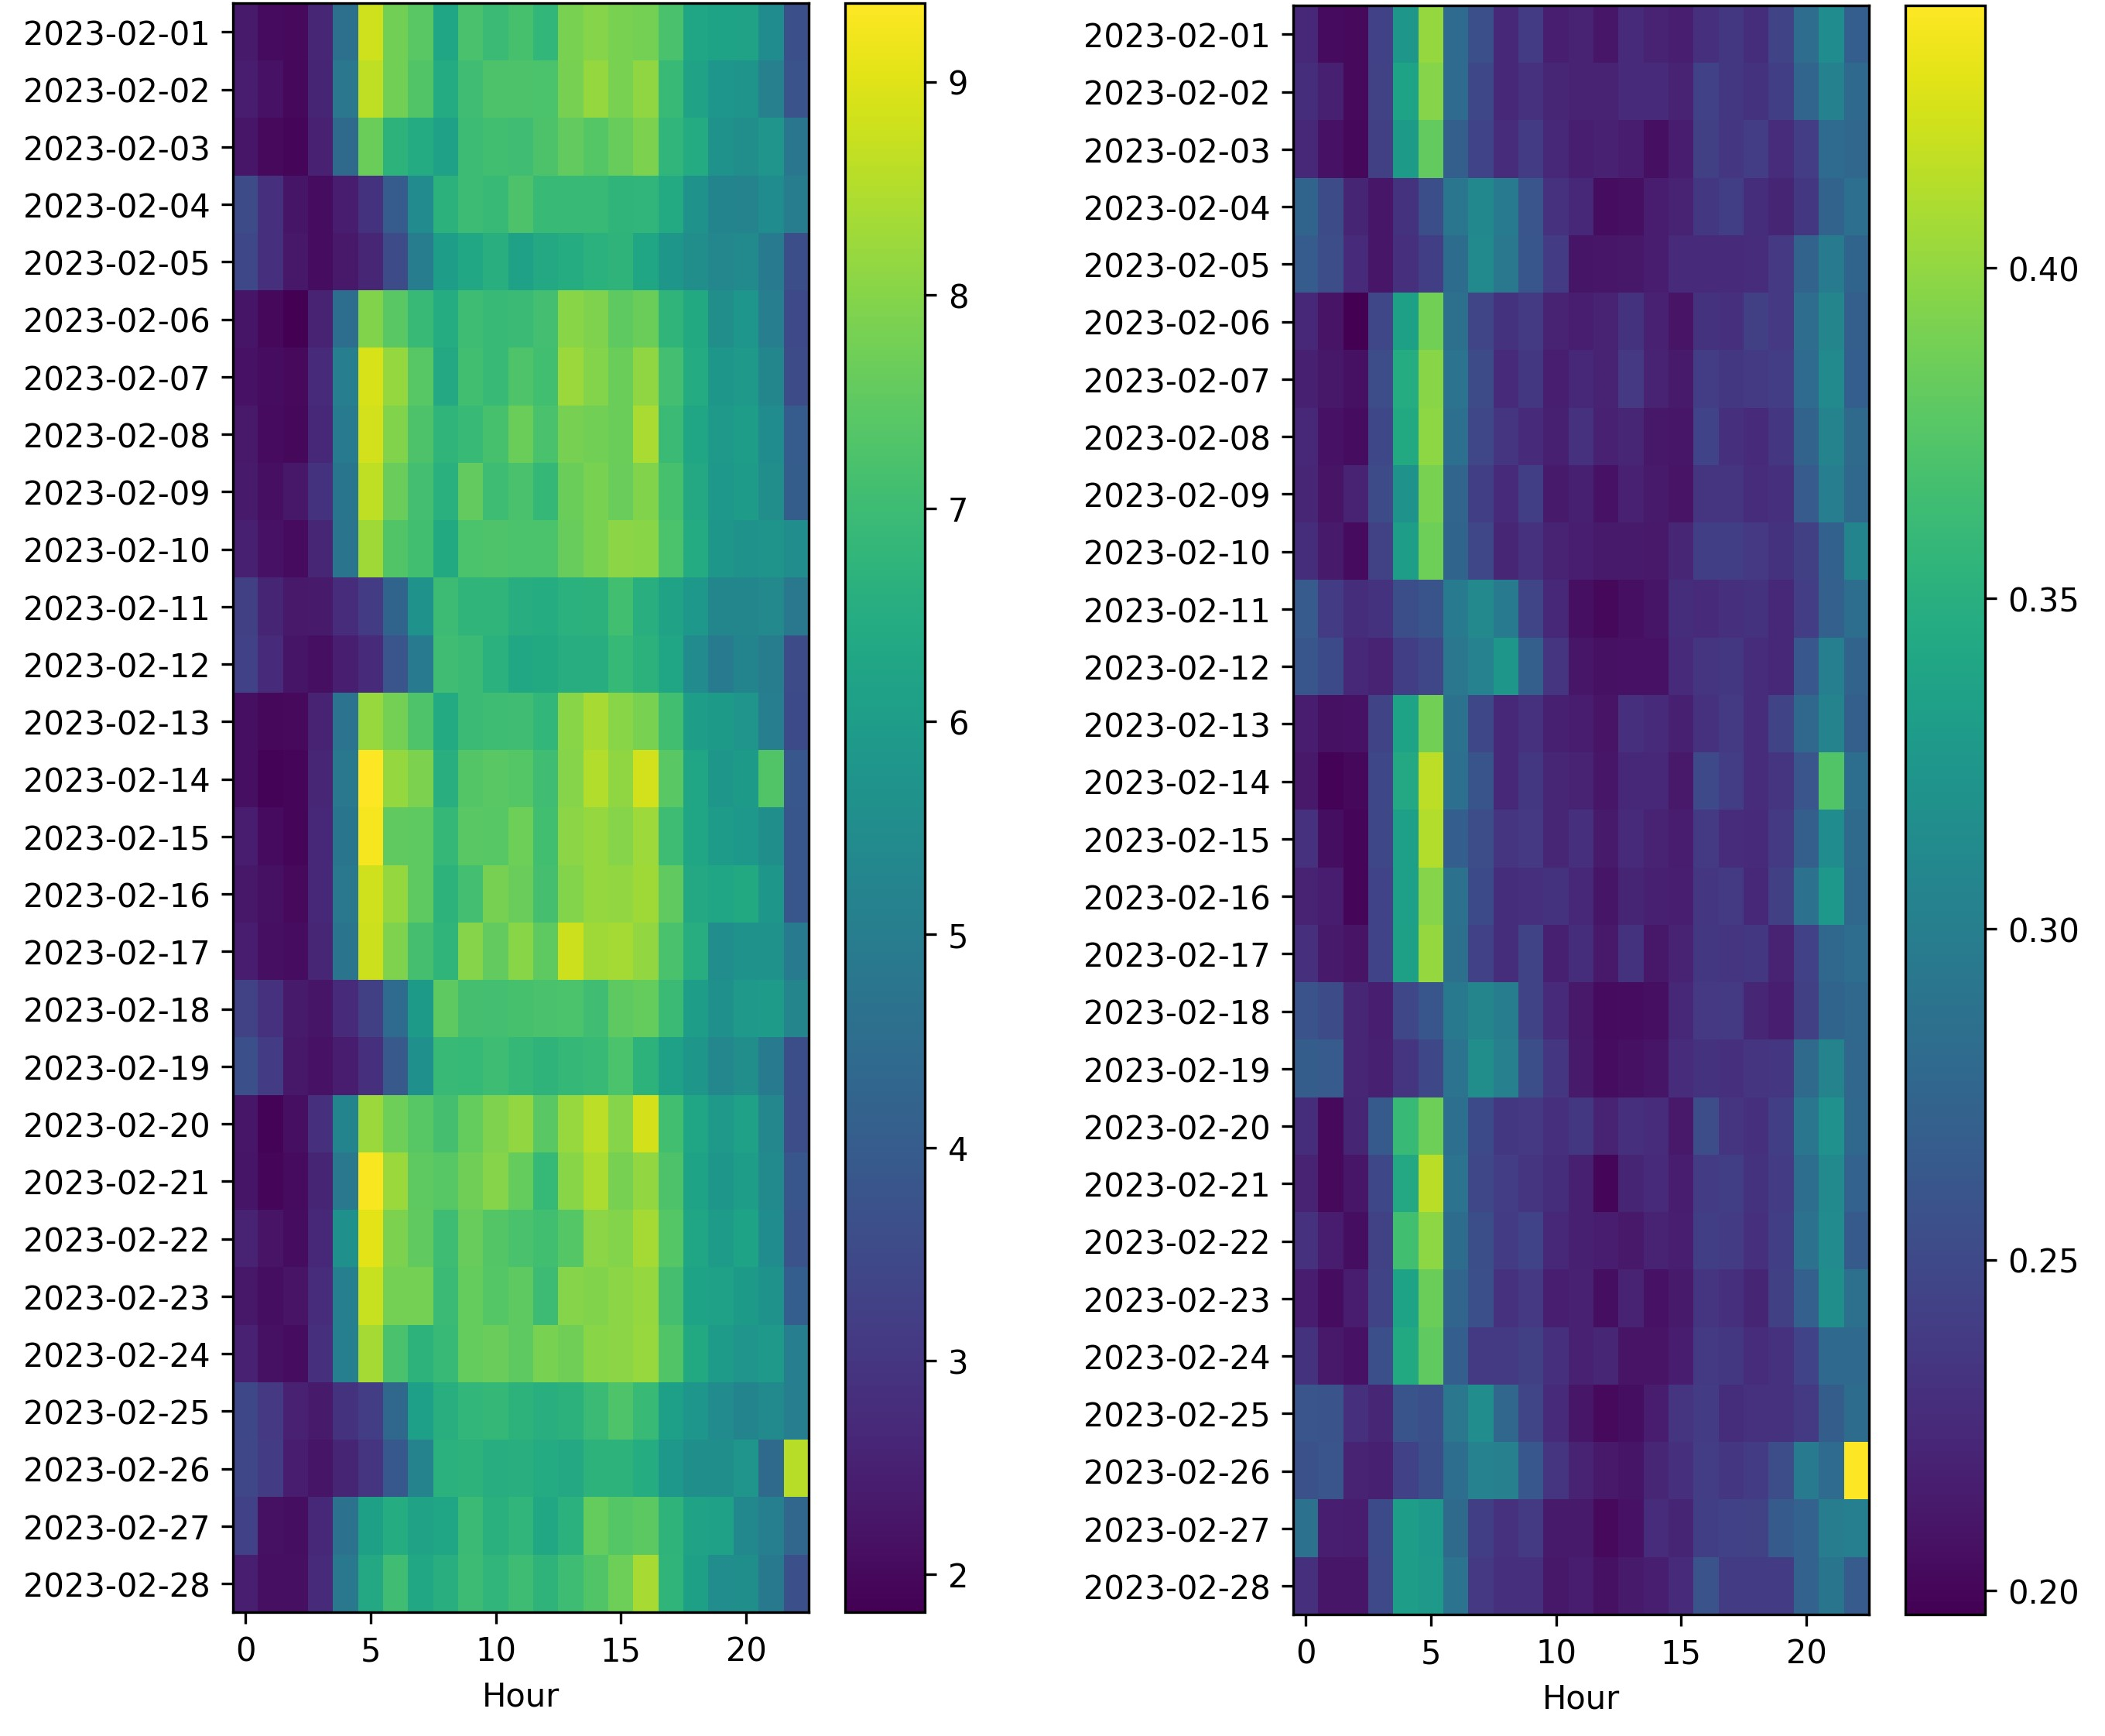
\includegraphics[width=1.6\textwidth]{graphics/results/new_L1_Jaccard_Feb.png}
\end{adjustbox}
\caption{Movement profiles for February 2023 using L1 (left) and Weighted Jaccard (right).}
\label{fig:mov-pro-feb}
\end{figure*}

\begin{figure*}[ht]
\centering
\begin{adjustbox}{center}
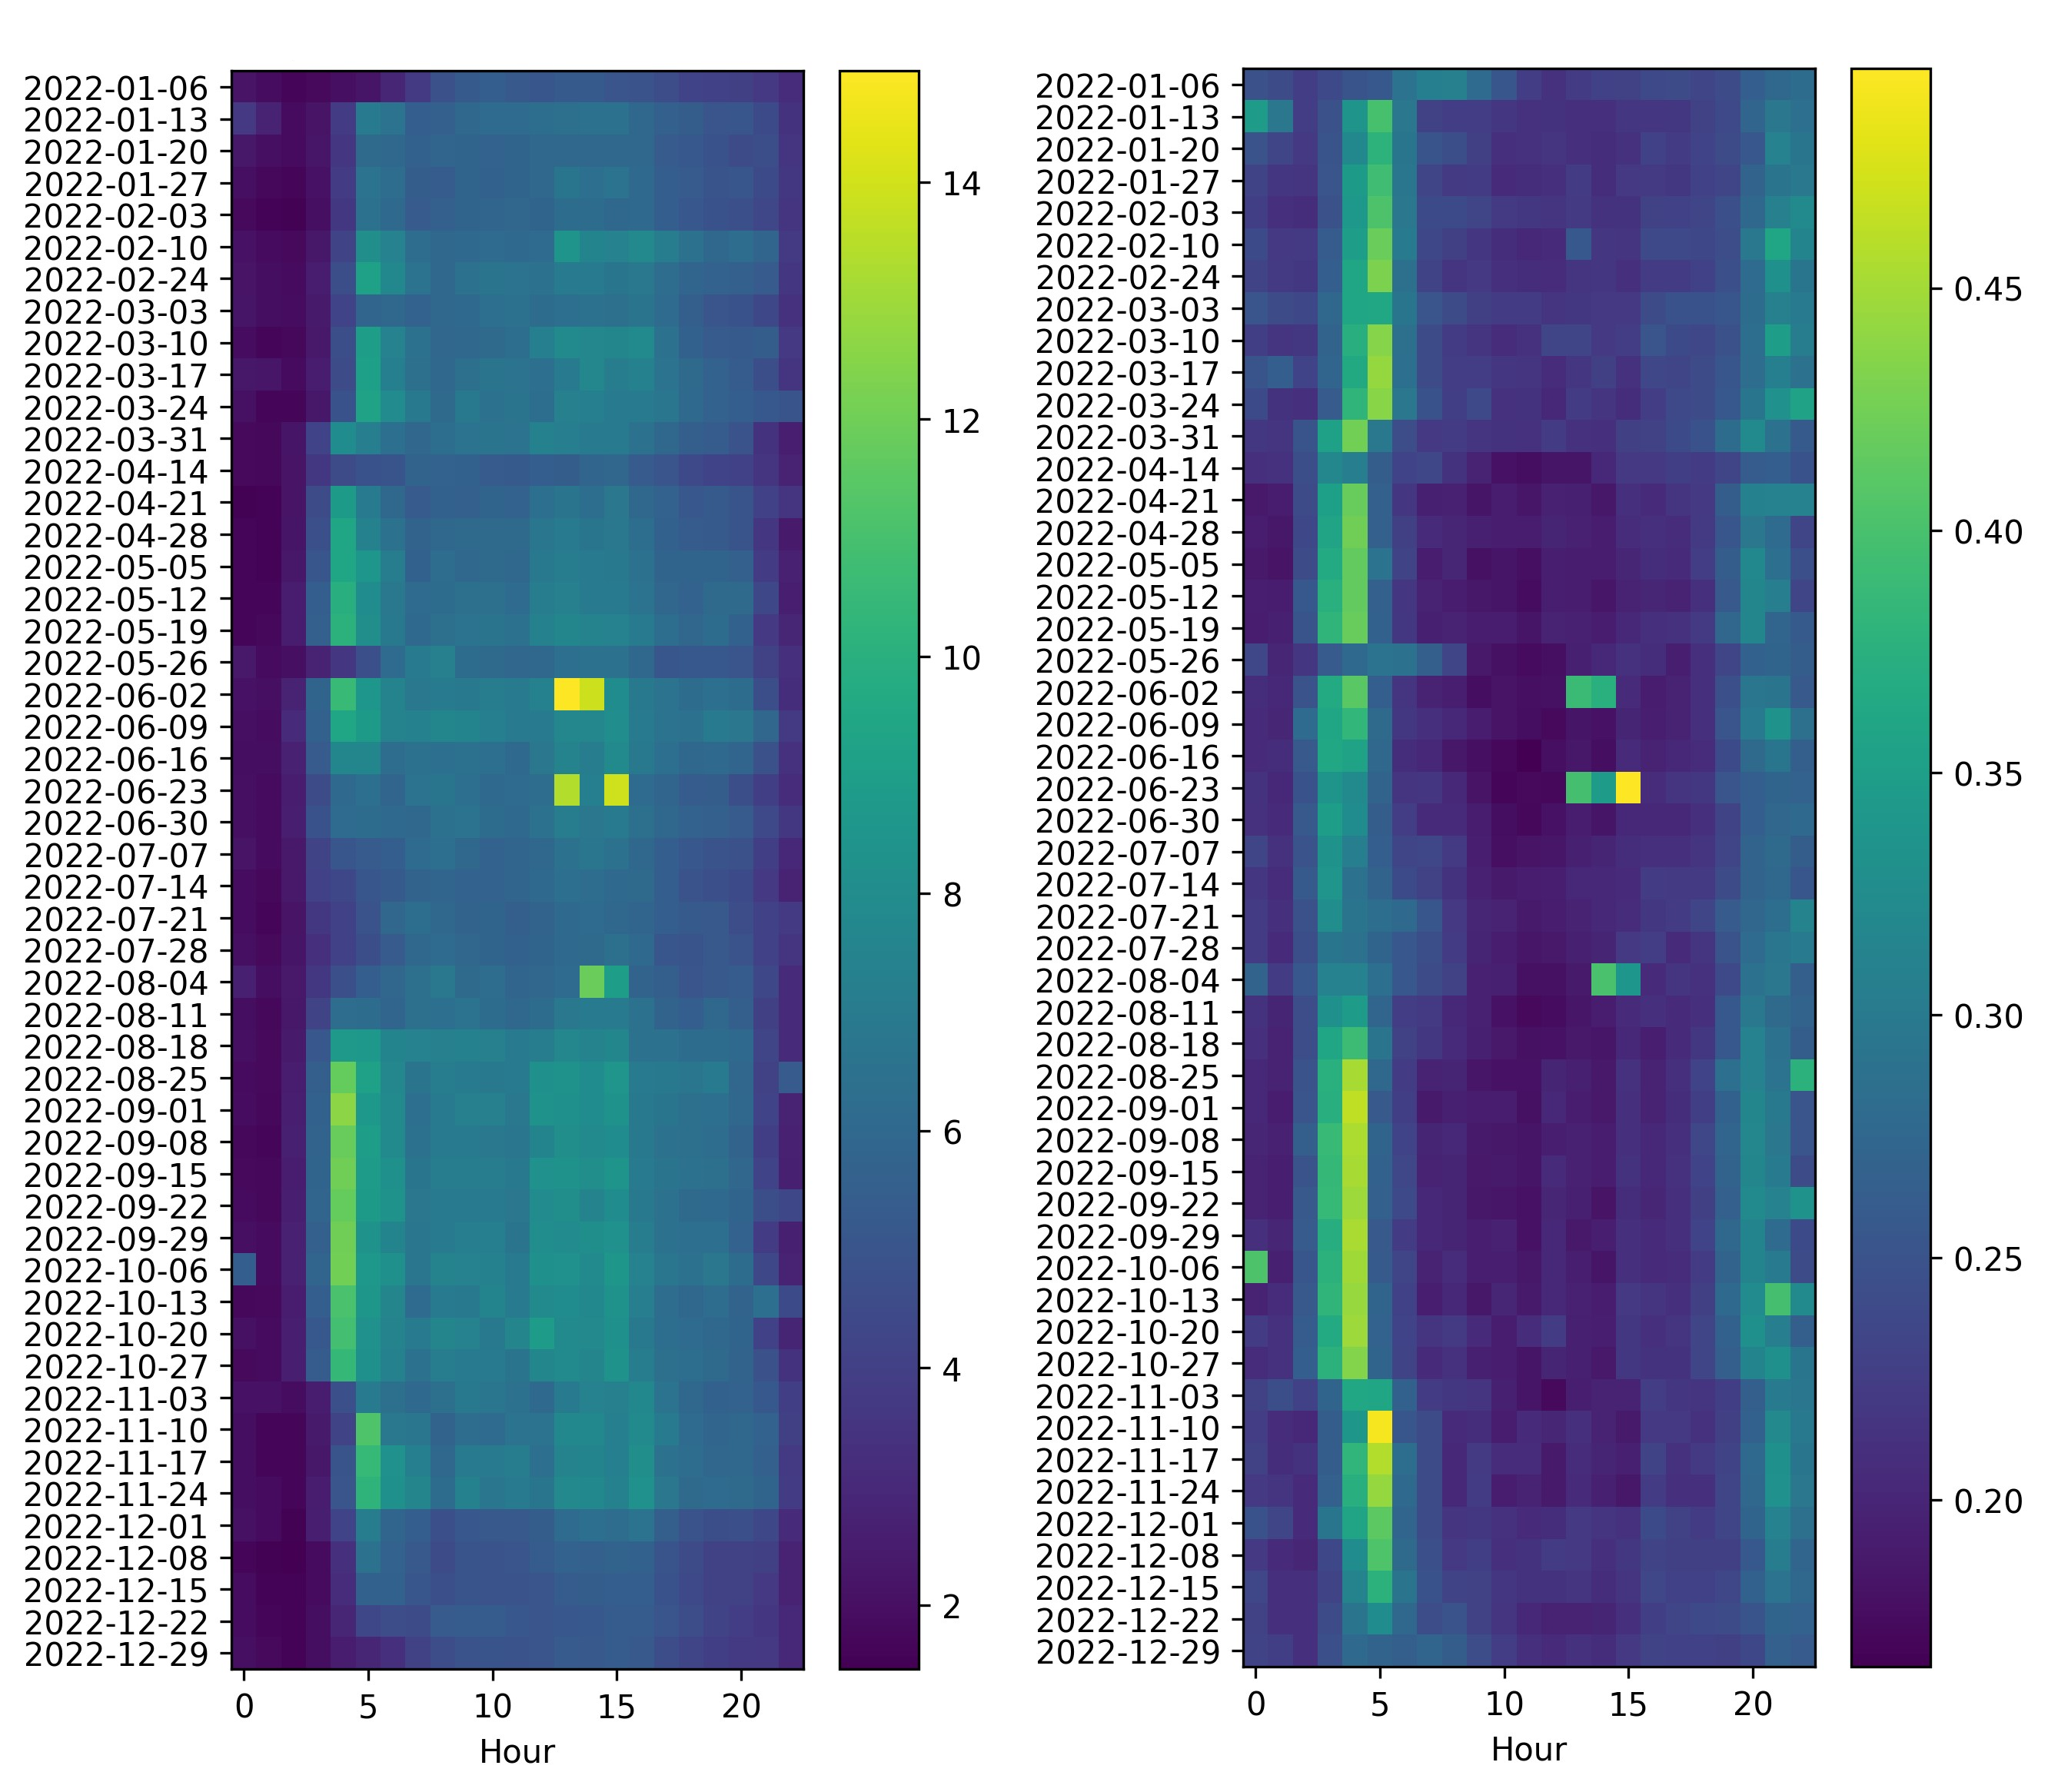
\includegraphics[width=1.6\textwidth]{graphics/results/new_L1_Jaccard_Year.png}
\end{adjustbox}
\caption{Movement profiles for Thursdays 2022 using L1 (left) and Weighted Jaccard (right).}
\label{fig:full-mov-pro}
\end{figure*}

\begin{figure*}[ht]
\vspace{-40mm}
\centering
\begin{adjustbox}{center}
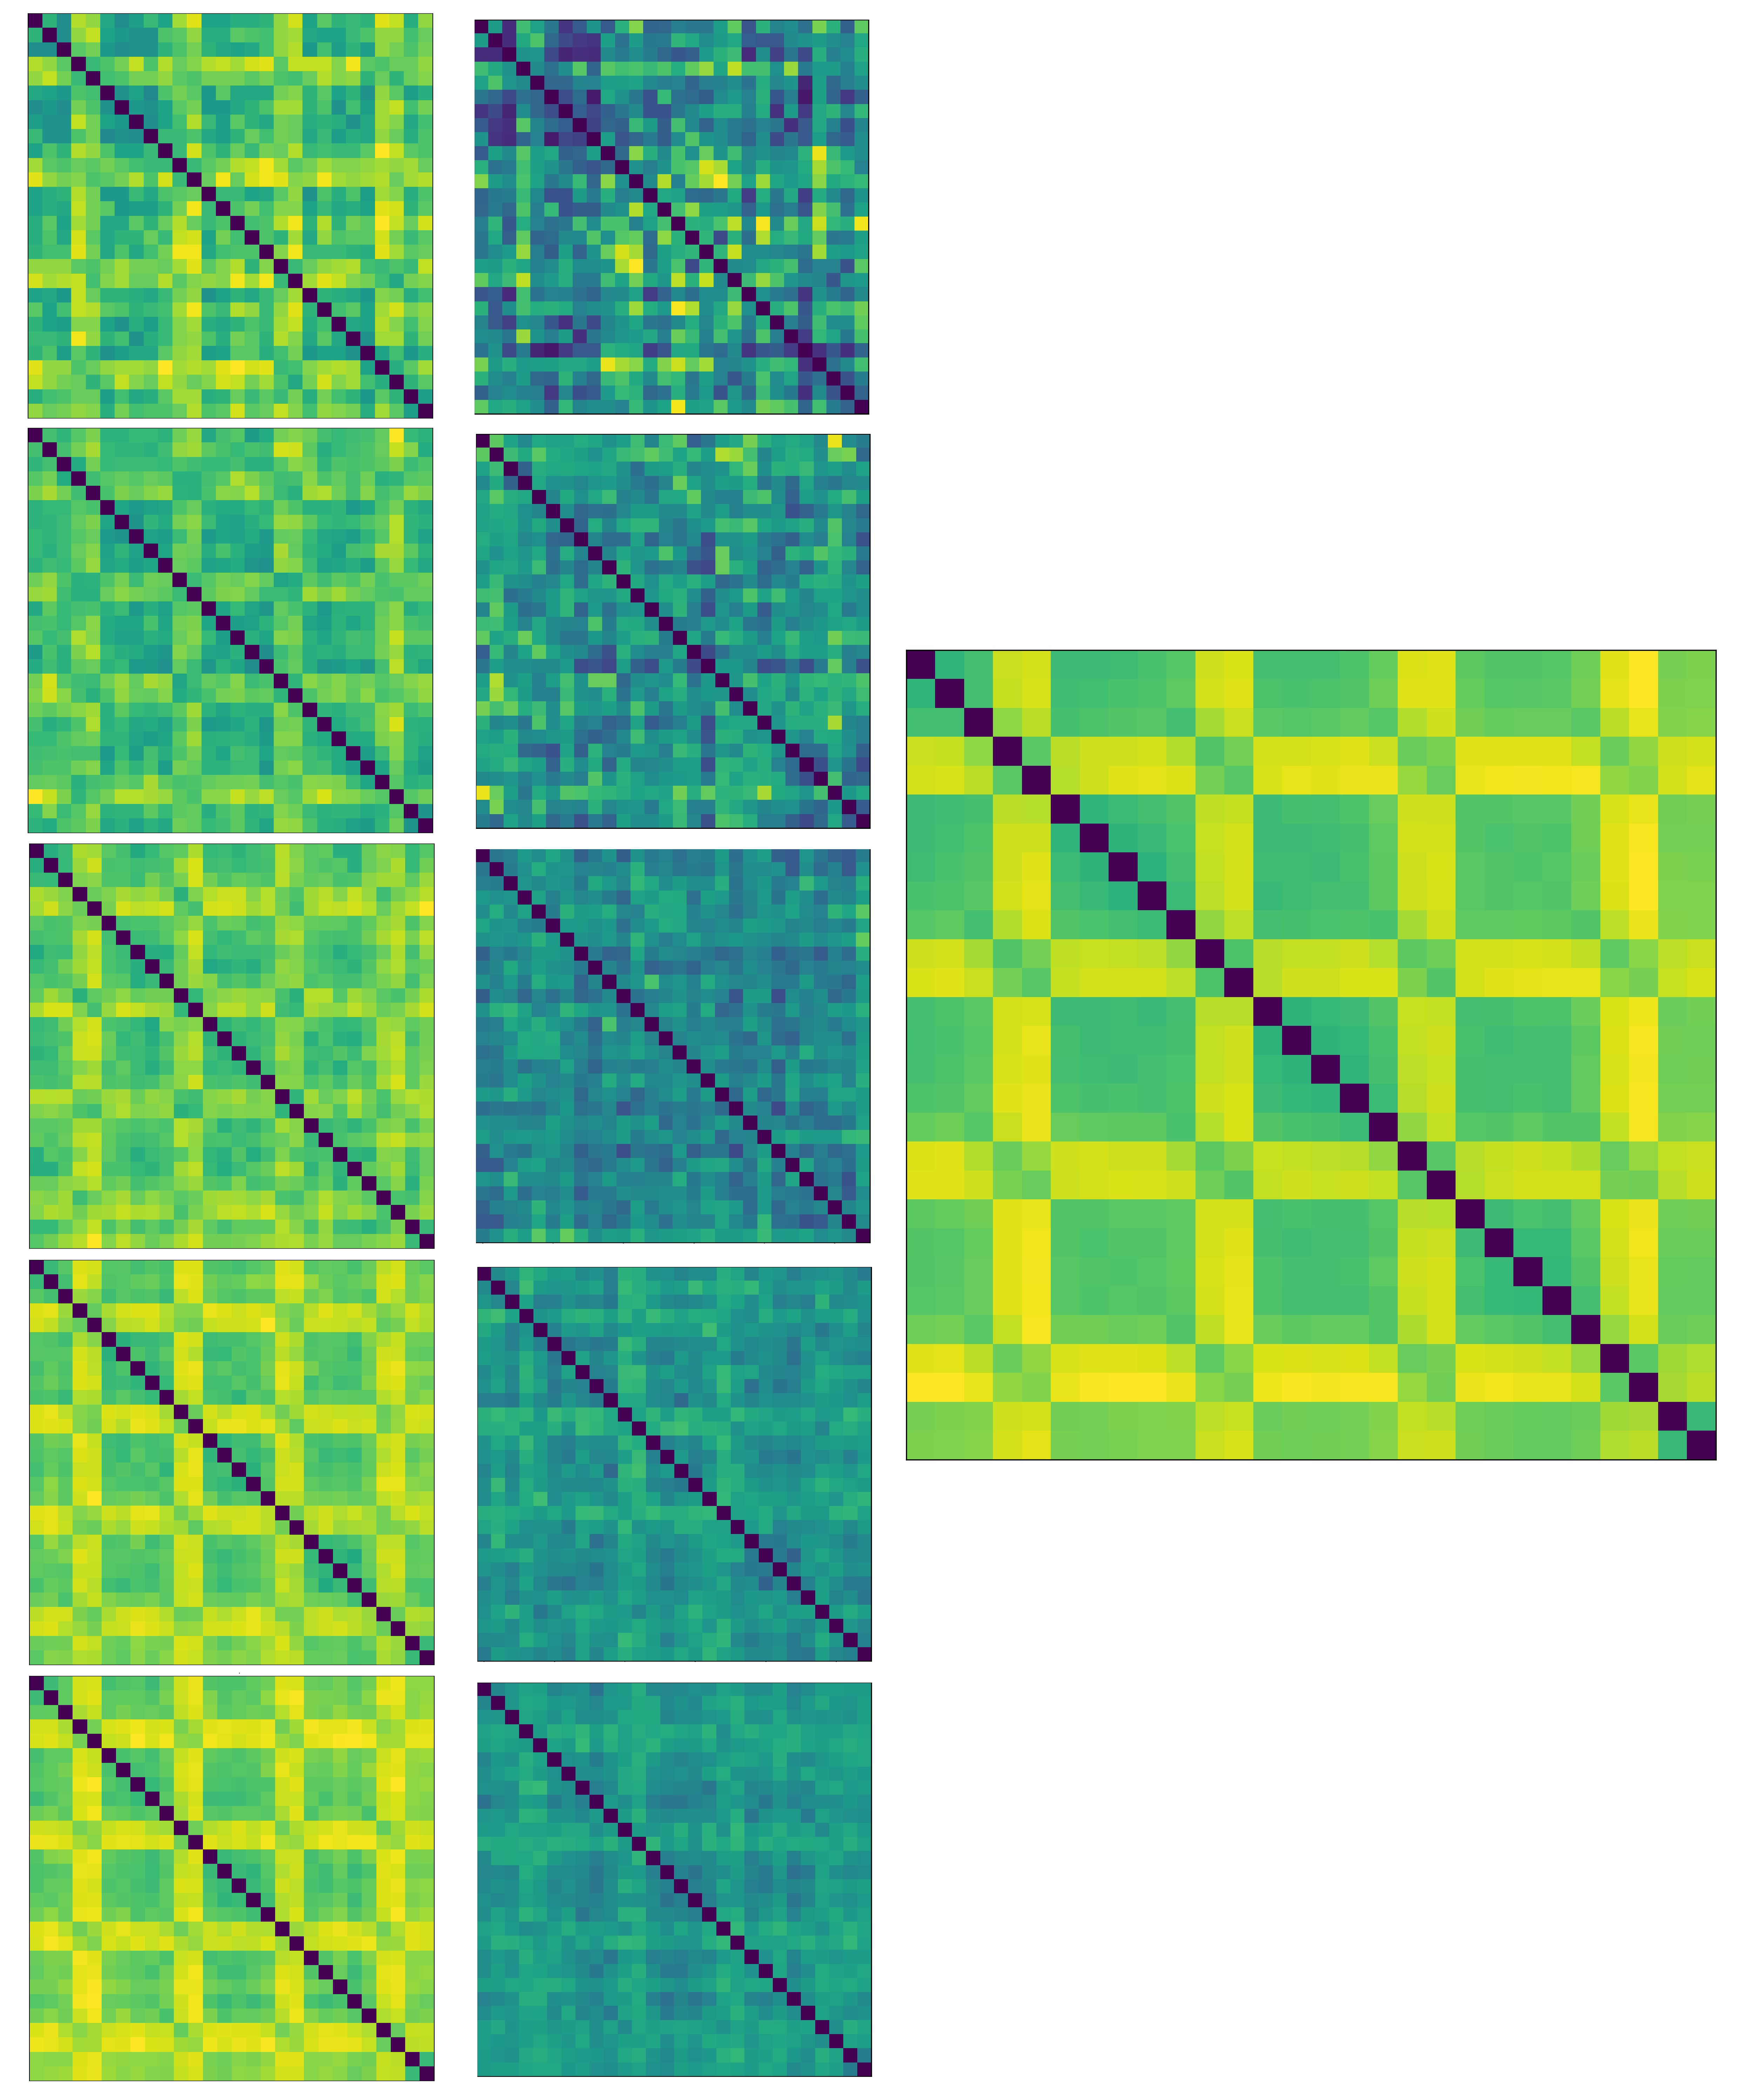
\includegraphics[width=1.4\textwidth]{graphics/results/comparison_minhash.png}
\end{adjustbox}
\caption{Comparisons of MinHash sampler rates. The left column shows the February distance matrix for difference sample rates: 64, 128, 256, 512 and 1024 from top to bottom. The middle column shows the element-wise difference between the MinHash matrix and the weighted Jaccard Distance (right).}
\label{fig:comparison_minhash}
\end{figure*}

\end{document}